\section{Random Walk on Networks}

The study of random walks on networks is fundamental in understanding various dynamical processes, such as diffusion, search algorithms, and transport phenomena. In this section, we formalize the mathematical framework of random walks on networks and explore their key properties, including stationary distributions, transition probabilities, and their connection to the Laplacian matrix.

Consider a network $G(N,M)$ where a particle moves randomly between the nodes at each time step, with transition probability $P_{ij}^{\Delta t}$ to go to the node $j$ starting from the node $i$ after a time interval $\Delta t$. If the link between them does not exist then $P_{ij}^{\Delta t}= 0$. 
The dynamics of this system is a Markov chain: it has no memory of the past states and the future state depends only on the current position.
Let $\rho_i(t)$ be the probability of finding the particle at the node $i$ at time $t$. The discrete time evolution of the system is given by the law
\begin{equation}\label{discrite random walk}
    \rho_i(n+\Delta t) = \sum_j P_{ij}^{\Delta t}\rho_j(n).
\end{equation}

In order to conserve the total probability the transition probability must be a stochastic matrix, namely it must hold 
\begin{equation}
    \sum_i P_{ij}^{\Delta t} = 1 .
\end{equation}

We define a regular random walk when
\begin{align}
    P^{\Delta t}_{ij}&=\pi_{ij}\Delta t + o(\Delta t) \qquad i\ne j\\
    P^{\Delta t}_{jj}&=1-\sum_{k\ne j}P^{\Delta t}_{kj}
\end{align}
where $\pi_{ij}$ are the transition rates, namely the transition probability per units of time, we set $\pi_{ii}=0$.
In un unweighted network, the transition rates can be identified with the adjacency matrix as
\begin{equation}
    \pi_{ij} = \frac{A_{ij}}{\sum_j A_{ij}}.
\end{equation}

Taking the continuum limit of the evolution \eqref{discrite random walk} we obtain the master equation \cite{Classic_random_walk}
\begin{equation}\label{master_eq}
    \dot \rho_i(t) = \sum_j \pi_{ij}\rho_j(t) - \pi_{ji}\rho_i(t) = - \sum_j L_{ij} \rho_j(t),
\end{equation}
where $L_{ij} = \sum_k \pi_{kj}\delta_{ij} -\pi_{ij} $ is the Laplacian matrix.
The first term represents incoming transitions to node $i$, while the second term accounts for outgoing transitions.

The Laplacian matrix has the property that $L_{ij} < 0 $ for $i \neq j$ and also it satisfies the relation
\begin{equation}
    \sum_i L_{ij} = 0 .
\end{equation} 

The eigenvalues of the Laplacian matrix have always a not negative real part and its spectrum contains at least one zero eigenvalue, therefore it is not invertible \cite{Boccaletti}. The multiplicity of the zero eigenvalue is equal to the number of connected component of the network: in fact that if the network is not connected the Laplacian should be a block matrix,  block for each connected component, each component can be seen as an independent network with their zero eigenvalue.

The solution of master equation \eqref{master_eq} is
\begin{equation}\label{random_walk_solution}
    \rho(t) = e^{-tL}\rho(0).
\end{equation}

We can prove that
\begin{equation}
    \sum_i \dot\rho_i(t) = - \sum_i \sum_j L_{ij} \rho_j(t) = - \sum_j \left(\sum_i L_{ij}\right) \rho_j(t) = 0 .
\end{equation}
This implies a first integral of motion 
\begin{equation}
    \sum_i \rho_i(t) = \sum_i \rho_i(0) .
\end{equation}

If the network is irreducible the master equation \eqref{master_eq} has a unique stationary solution $\rho^*$ that satisfies
\begin{equation}
    \sum_j (\pi_{ij}\rho_j^\ast-\pi_{ji}\rho_i^\ast)=-\sum_j J^*_{ij}=0
\end{equation}
where we introduce the stationary density currents $J^*_{ij} = \pi_{ji}\rho_i^\ast-\pi_{ij}\rho_j^\ast $.
The stationary density currents $J_{ij}^\ast$ vanishes and the vector field on the network
$$
v_{ij}=\ln \pi_{ij}-\ln \pi_{ji}
$$
is exact and it admits a potential $V_i$ such that
$$
v_{ij}=V_j-V_i\qquad \forall \; (i,j)
$$
The stationary distribution can be written in the form
\begin{equation}
    \label{MB}
    \rho_i^\ast \propto \exp(-V_i)
\end{equation}
and one recovers the MB distribution according to MEP.

If Laplacian is symmetric the system admits a unique stationary solution \cite{Classic_random_walk} 
\begin{equation}\label{ones_vector}
    \rho^* = \frac{1}{N} \left(1,1,\cdots,1,1\right).
\end{equation} 
such that
\begin{equation}
    \sum_j L_{ij}\rho^*_j =  0.
\end{equation}
Thus, the stationary distribution \eqref{ones_vector} is the eigenvector with eigenvalue $0$ of the Laplacian matrix. 

We can consider a less strict condition for the system known as detailed balance condition
\begin{equation}\label{detail_condition}
    \pi_{ij} \rho_j^* = \pi_{ji} \rho_i^*,
\end{equation}
in other word, each current $J^*_{ij}$ vanishes.
In this case, the Laplacian matrix can be reduced to a symmetric matrix 
\begin{equation}
    S_{ij}=\frac{1}{\sqrt{\rho_i^\ast}}L_{ij}\sqrt{\rho_j^\ast},
\end{equation}
so that the eigenvalues are real and the eigenvectors are orthogonal. In particular \eqref{ones_vector} is the zero eigenvector of $S_{ij}$ and the master equation reads 
\begin{equation}
    \tilde p_i=-\sum_j S_{ij} \tilde p_j
\end{equation}
where $\tilde p_i=p_i\sqrt{\rho_i^\ast}$. 

.
%The other eigenvalues are connected to the Ljapunov exponent and to the time that the occurs to converge to $\rho^*$.

Let us now assume the network satisfies the detailed balance condition \eqref{detail_condition}, then there exists a hyperplane $\Sigma_0$ that is orthogonal to the stationary distribution and this subspace is invariant under the dynamics. Let be $w \in \Sigma_0$, this subspace is identify by the relation
\begin{equation}
    \sum_i w_i = 0.
\end{equation}


Therefore, any probability vector can be decomposed as a direct sum of the stationary state and a vector $w(t) \in \Sigma_0$ 
\begin{equation}
    \rho(t) = \rho^* + w(t).
\end{equation}
Thus, all the eigenvectors with not zero eigenvalues belong to this subspace.


The uncertainty in the particle's location can be captured by the Shannon entropy
\begin{equation}
    S = -\sum_i p_i\ln p_i.
\end{equation}
It is a bounded function $0\geq S \geq \ln N$.
It can been shown that the stationary distribution maximizes the Shannon entropy $S = \ln N$.
    
\begin{comment}
    In figure \ref{fig:node_0} is shown only the probability to be in the initial node as a function of time starting  from a Dirac delta distribution for different types of networks\footnote{The python scripts can be found in the GitHub page of the author at the link: \url{https://github.com/ShqemzaMatteo/Master_thesis}}: a ring graph, an Erd\H{o}s-Rényi (E-R) random graph\cite{erdos-renyi1960}, a Barab\'asi-Albert (B-A) scale-free graph\cite{Barabasi_Albert_1999}, and a Watts-Strogatz (W-S) small-sworld graph\cite{Watts-Strogatz_1998}. All the algorithm are explained in the Appendix \Ref{Appendix_A}. 

    \begin{figure}[ht!]
        \centering
        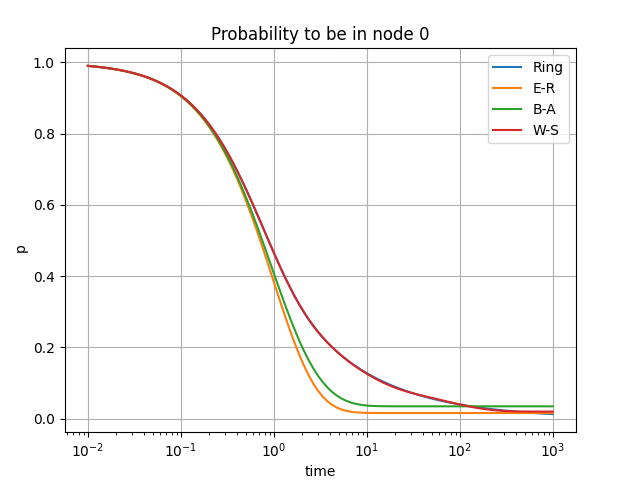
\includegraphics[width=0.65\linewidth]{image/random_graph_node_0.png}
        \caption{Plot of the probability $p$ to be in the node 0 starting from a Dirac delta distribution or the same node as a function of time for different network types of $50$ nodes: a ring graph (blue), a Erd\H{o}s-Rényi (E-R) random graph with connectivity probability $0.7$ (orange), a Barab\'asi-Albert (B-A) scale-free graph with parameter $m=3$ (green), and a Watts-Strogatz (W-S) small world graph with parameter $K=3$ and rewire probability 0.2 (red).}
        \label{fig:node_0}
    \end{figure}
\end{comment}